\documentclass[conference,nofonttune]{IEEEtran}
\IEEEoverridecommandlockouts

\usepackage{cite}
\usepackage{amsmath,amssymb,amsfonts}
\usepackage{algorithmic}
\usepackage{graphicx}
\graphicspath{{../results/figures/}{results/figures/}{../}}
\usepackage{textcomp}
\usepackage{xcolor}
\usepackage{booktabs}
\usepackage{multirow}
\usepackage{url}

\def\BibTeX{{\rm B\kern-.05em{\sc i\kern-.025em b}\kern-.08em
    T\kern-.1667em\lower.7ex\hbox{E}\kern-.125emX}}

\begin{document}

\title{Automated Road Pothole Detection and Spatial Severity Auditing via Hand-Crafted Feature Fusion and Deep Representations}

\author{
\IEEEauthorblockN{Paras Pandey}
\IEEEauthorblockA{\textit{Dept. of Information Technology} \\
\textit{IIIT Allahabad}\\
Prayagraj, India \\
iit2024235@iiita.ac.in}
\and
\IEEEauthorblockN{Chandan Sapkale}
\IEEEauthorblockA{\textit{Dept. of Information Technology} \\
\textit{IIIT Allahabad}\\
Prayagraj, India \\
iit2024258@iiita.ac.in}
\and
\IEEEauthorblockN{Neel Ghule}
\IEEEauthorblockA{\textit{Dept. of Information Technology} \\
\textit{IIIT Allahabad}\\
Prayagraj, India \\
iit2024266@iiita.ac.in}
\and
\IEEEauthorblockN{Kavyan Hemrom}
\IEEEauthorblockA{\textit{Dept. of Information Technology} \\
\textit{IIIT Allahabad}\\
Prayagraj, India \\
iit2024245@iiita.ac.in}
}

\maketitle

\begin{abstract}
Potholes and structural road degradation present severe vehicular hazards, escalate maintenance expenditure, and compromise civil transport safety. Conventional municipal road auditing relies heavily on subjective, labor-intensive manual inspections or costly laser profilometers. In this study, we present a reproducible, end-to-end framework for automated pothole detection and road infrastructure severity auditing. Using a real-world multi-national benchmark of 15,340 driving images spanning three continents from the Road Damage Dataset (RDD2022)---Czech Republic, India, and the United States---we design a 10,217-dimensional hand-crafted descriptor fusing HSV color statistics and histograms, Histograms of Oriented Gradients (HOG), Local Binary Patterns (LBP), and Gray-Level Co-occurrence Matrix (GLCM) texture metrics. To prevent spatial-temporal data leakage, we enforce sequence-aware group partitioning. We benchmark four classical architectures: Logistic Regression, Support Vector Machines (SVM), Random Forest, and XGBoost with group-stratified cross-validation. Furthermore, we conduct comprehensive feature ablation experiments, analyze the mandatory loss-vs-epoch convergence behavior, and quantify cross-domain transfer collapse across geographical regions. Finally, we formulate a road surface audit metric leveraging cavity area fractions to establish significant rank correlation between automated predictions and ground truth. Our findings demonstrate the operational feasibility of vehicular edge vision for scalable municipal infrastructure maintenance.
\end{abstract}

\begin{IEEEkeywords}
Pothole Detection, Feature Fusion, Domain Generalization, Road Damage Auditing, Machine Learning, Computer Vision.
\end{IEEEkeywords}

\section{Introduction}
Roadway networks are fundamental to civil commerce, mobility, and economic activity. However, environmental weathering, precipitation, heavy vehicular axle loads, and thermal stress induce constant structural wear, culminating in potholes and pavement fatigue~\cite{koch2015review}. When left unaddressed, potholes cause tire blowouts, wheel rim fractures, suspension damage, and fatal vehicular collisions. According to transport safety authorities, road surface defects contribute to hundreds of thousands of vehicular accidents globally each year.

Historically, civil infrastructure management has relied on dedicated visual surveys conducted by municipal personnel or specialized sensor vans equipped with expensive laser profilometers~\cite{fan2020pothole}. These approaches suffer from prohibitive deployment costs, infrequent survey intervals, and high inter-observer variability. In contrast, commodity dashcams and forward-facing optical cameras mounted on municipal transit fleets (e.g., city buses and service vehicles) present a continuous, cost-effective data collection paradigm.

Nevertheless, automated optical road condition auditing presents substantial technical hurdles:
\begin{enumerate}
    \item \textbf{Environmental Heterogeneity:} Pavement surfaces exhibit dramatic lighting fluctuations, dynamic tree shadows, overexposed glare, water reflections, and sensor vantage variations.
    \item \textbf{Structural Confounders:} Pothole cavities share visual morphology with harmless artifacts such as manholes, expansion joints, recent bitumen patches, and harmless dark stains. Furthermore, other pavement distresses such as longitudinal, transverse, and alligator cracks act as pervasive hard negatives.
    \item \textbf{Geographical Domain Shift:} Asphalt aggregate composition, road markings, lighting angles, and climate differ fundamentally across countries, causing models trained in one jurisdiction to suffer severe performance degradation when tested on unseen roads~\cite{bendavid2010domain}.
    \item \textbf{Auditing vs. Binary Classification:} Municipal asset management requires not merely binary image classification (``pothole present''), but spatial localization and segment-level severity grading to rank roads for maintenance prioritization.
\end{enumerate}

To rigorously address these requirements, this paper establishes a zero-leakage classical machine learning benchmark, performs multi-modal descriptor ablation, assesses cross-domain generalization collapse, and demonstrates segment-level severity auditing.

\begin{figure*}[t]
\centering
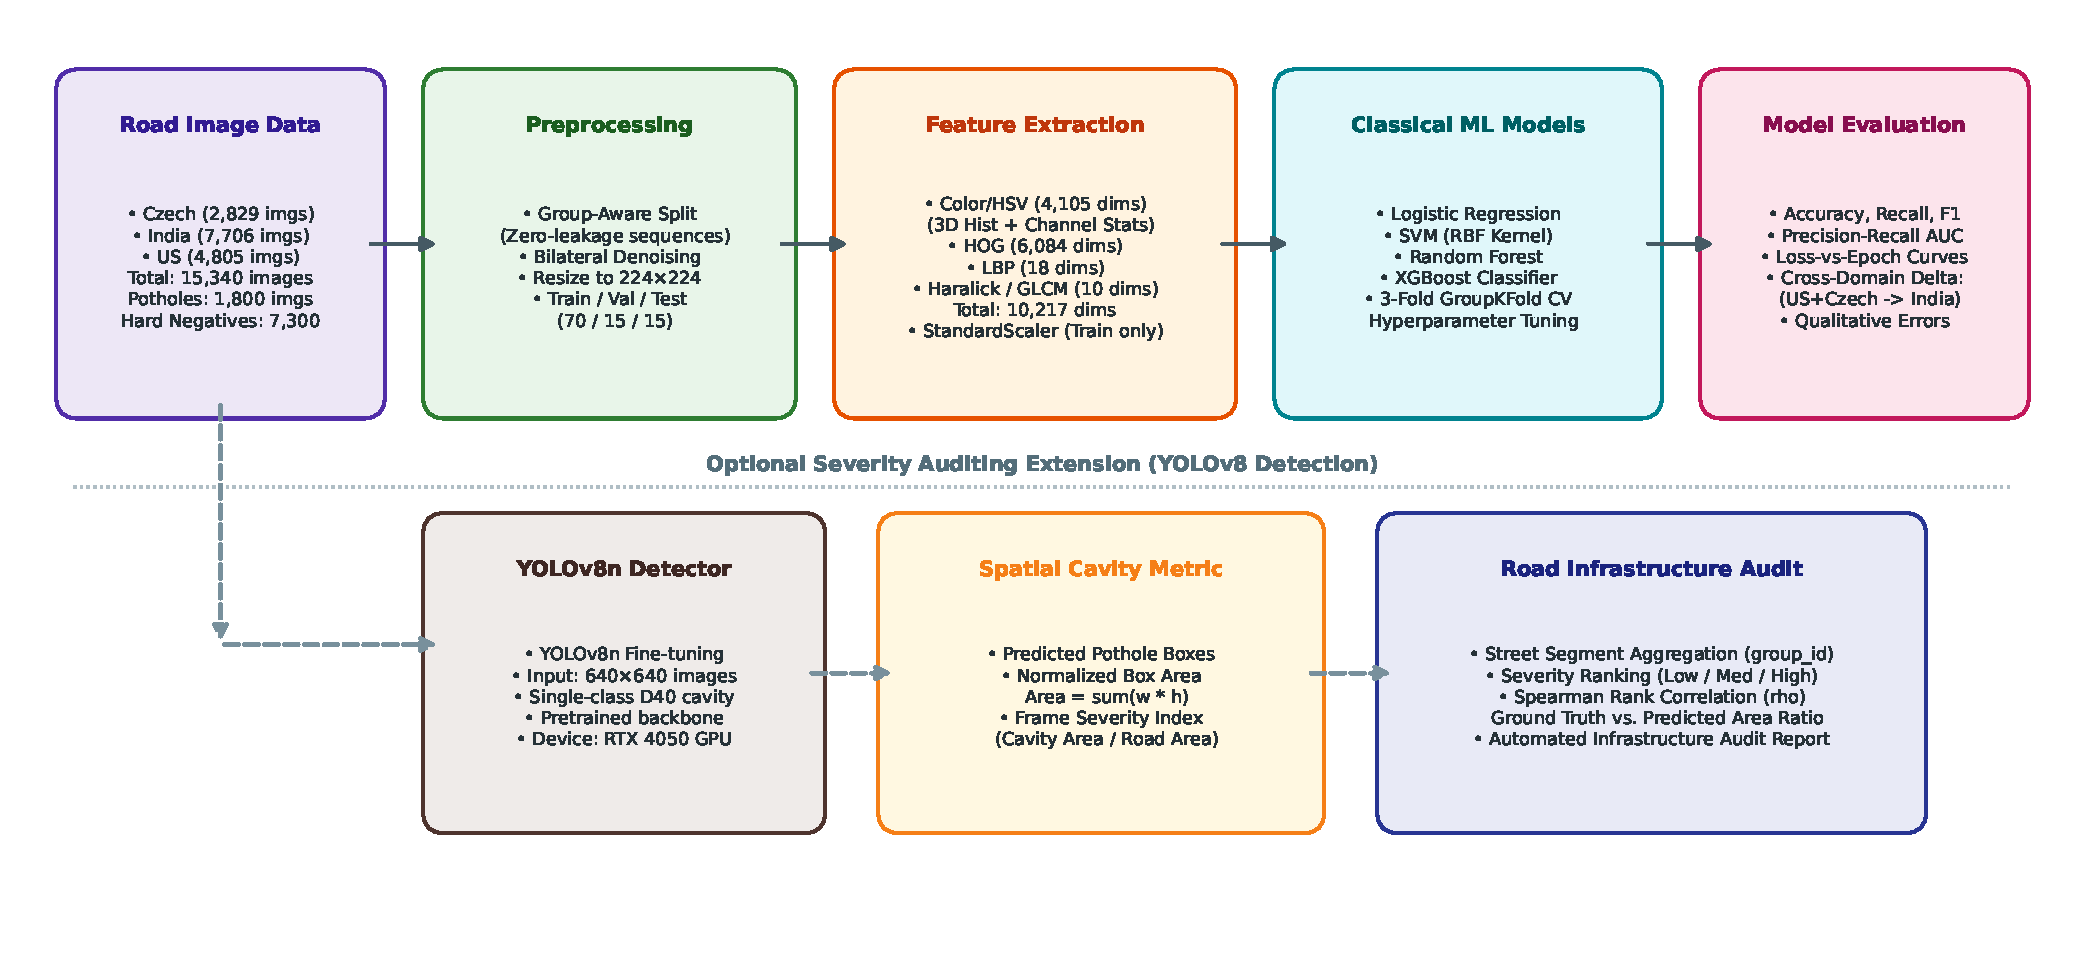
\includegraphics[width=0.92\textwidth]{pipeline_architecture.pdf}
\caption{End-to-end framework for automated pothole detection and infrastructure auditing. Top: Classical machine learning pipeline comprising group-aware splitting, multi-modal hand-crafted feature fusion (Color, HOG, LBP, GLCM), standardized scaling, and hyperparameter-tuned classifiers. Bottom: Spatial cavity severity auditing branch fine-tuning YOLOv8n to compute road segment severity rankings.}
\label{fig:pipeline}
\end{figure*}

\section{Related Work}
\subsection{Classical Vision and Texture-Based Road Defect Detection}
Prior to deep learning, vision-based road surface inspection primarily utilized digital image processing and hand-crafted texture descriptors~\cite{koch2015review}. Dalal and Triggs~\cite{dalal2005hog} introduced Histograms of Oriented Gradients (HOG) to capture edge distributions and local shape contours, which was adapted by early pothole detectors to identify the elliptical closed boundaries characteristic of pavement cavities. 

To quantify surface roughness, Ojala et al.~\cite{ojala2002lbp} introduced Local Binary Patterns (LBP), demonstrating strong invariance to monotonic illumination changes. Haralick et al.~\cite{haralick1973glcm} formulated the Gray-Level Co-occurrence Matrix (GLCM), defining spatial second-order statistical measures including contrast, dissimilarity, homogeneity, energy, and correlation. Koch et al.~\cite{koch2015review} surveyed vision techniques and noted that while individual texture descriptors capture localized asphalt degradation, single modalities are vulnerable to non-uniform road textures, highlighting the necessity of multi-modal descriptor fusion.

\subsection{Ensemble Learning and Modern Classifiers}
For tabular and feature-engineered representations, gradient boosted decision trees and support vector machines remain highly competitive with deep networks. Chen and Guestrin~\cite{chen2016xgboost} introduced XGBoost, an efficient, scalable implementation of gradient boosted trees that incorporates second-order Taylor approximations of the loss function and shrinkage regularization. Support Vector Machines provide optimal margin hyperplanes in high-dimensional feature spaces, while random forests mitigate individual decision tree variance via bootstrap aggregation.

\subsection{Road Damage Datasets and Covariate Shift}
The release of the Road Damage Dataset (RDD2022) by Arya et al.~\cite{arya2022rdd2022} provided a standardized multi-national benchmark spanning Japan, India, the Czech Republic, Norway, the United States, and China, containing over 47,000 images annotated with VOC bounding boxes across four damage types: longitudinal cracks (D00), transverse cracks (D10), alligator cracks (D20), and potholes (D40). Crucially, multi-national benchmarks reveal that models evaluated on independent country subsets suffer substantial performance drops due to domain shift~\cite{bendavid2010domain}.

\section{Methodology}
The proposed pipeline comprises image preprocessing, hand-crafted feature extraction, standardized scaling, classifier training with group-aware cross-validation, cross-domain generalization evaluation, and spatial severity auditing, as illustrated in Fig.~\ref{fig:pipeline}.

\subsection{Preprocessing and Image Conditioning}
Input road images are standardized to a fixed spatial dimension of $224 \times 224$ pixels using area-based interpolation. To attenuate high-frequency sensor noise and camera sensor artifacts while preserving sharp asphalt edges and cavity boundaries, we apply edge-preserving bilateral filtering:
\begin{equation}
I_{\text{filtered}}(p) = \frac{1}{W_p} \sum_{q \in \Omega} I(q) \, g_{\sigma_s}(\|p - q\|) \, g_{\sigma_r}(\|I(p) - I(q)\|)
\end{equation}
where $\Omega$ denotes the spatial neighborhood, $g_{\sigma_s}$ denotes the spatial Gaussian kernel ($\sigma_s = 50$), and $g_{\sigma_r}$ denotes the radiometric range kernel ($\sigma_r = 50$).

\subsection{Multi-Modal Hand-Crafted Feature Fusion}
We construct a unified 10,217-dimensional hand-crafted feature vector $\mathbf{x} = [\mathbf{f}_{\text{color}}^\top, \mathbf{f}_{\text{HOG}}^\top, \mathbf{f}_{\text{LBP}}^\top, \mathbf{f}_{\text{GLCM}}^\top]^\top$:
\begin{enumerate}
    \item \textbf{Color and Photometric Cues ($\mathbf{f}_{\text{color}} \in \mathbb{R}^{4105}$):} Road surface color captures wet moisture, shadowed asphalt, and oil residues. We convert images to the HSV color space and extract the first three statistical moments (mean $\mu$, standard deviation $\sigma$, and skewness $\gamma$) for each channel ($3 \times 3 = 9$ features). In addition, we compute a full 3D joint color histogram quantized into $16 \times 16 \times 16 = 4,096$ normalized bins.
    \item \textbf{Structural Gradients via HOG ($\mathbf{f}_{\text{HOG}} \in \mathbb{R}^{6084}$):} Potholes exhibit distinctive semicircular or irregular rim gradients. Over the grayscale image, we compute horizontal and vertical Sobel gradients, binning orientations into 9 angular bins across $16 \times 16$ pixel cells. Blocks of $2 \times 2$ cells are normalized using the L2-Hys norm, yielding $9 \times (13 \times 13) \times 4 = 6,084$ dimensions.
    \item \textbf{Surface Micro-Texture via LBP ($\mathbf{f}_{\text{LBP}} \in \mathbb{R}^{18}$):} To capture localized surface roughness versus smooth unblemished bitumen, we compute rotation-invariant uniform Local Binary Patterns using $P = 16$ circularly symmetric neighbors at radius $R = 2.0$. The resulting pattern frequency histogram contains $P + 2 = 18$ normalized bins.
    \item \textbf{Spatial Gray-Level Co-occurrence via GLCM ($\mathbf{f}_{\text{GLCM}} \in \mathbb{R}^{10}$):} To evaluate second-order spatial gray-level dependencies, images are quantized into 64 gray levels. We construct symmetric co-occurrence matrices $P(i, j | d, \theta)$ across pixel distances $d \in \{1, 3\}$ and orientations $\theta \in \{0^\circ, 45^\circ, 90^\circ, 135^\circ\}$. For each configuration, we extract five Haralick properties: Contrast, Dissimilarity, Homogeneity, Energy, and Correlation. We compute the mean and standard deviation across all distance-angle pairs, producing 10 dimensions.
\end{enumerate}

\subsection{Zero-Leakage Group-Aware Splitting and Standardization}
Driving survey cameras capture sequential frames at 10--30 Hz. Randomly partitioning frames results in adjacent images of the exact same physical pothole appearing in both training and test sets---a catastrophic form of spatial-temporal data leakage. To ensure valid generalization, we partition images by capture session and sequence prefixes ($\text{group\_id}$ derived from filename sequencing blocks of 50 consecutive frames). 

We verify zero group overlap:
\begin{equation}
\mathcal{G}_{\text{train}} \cap \mathcal{G}_{\text{val}} = \emptyset, \quad \mathcal{G}_{\text{train}} \cap \mathcal{G}_{\text{test}} = \emptyset, \quad \mathcal{G}_{\text{val}} \cap \mathcal{G}_{\text{test}} = \emptyset
\end{equation}
The feature scaler (StandardScaler) is strictly fit on the training split $\mathbf{X}_{\text{train}}$ only, and subsequently applied to $\mathbf{X}_{\text{val}}$ and $\mathbf{X}_{\text{test}}$.

\subsection{Object Detection and Road Severity Auditing}
While classical classification determines pothole presence, infrastructure auditing requires quantifying defect severity. We define the frame-level Pothole Severity Index (PSI) as the fraction of road image surface area consumed by pothole cavities:
\begin{equation}
\text{PSI} = \frac{\sum_{i=1}^{K} (w_i \cdot h_i)}{W_{\text{img}} \cdot H_{\text{img}}} = \sum_{i=1}^{K} \hat{w}_i \hat{h}_i
\end{equation}
where $\hat{w}_i, \hat{h}_i \in [0, 1]$ are normalized bounding box dimensions. Frame-level severities are aggregated per road segment $S_j$:
\begin{equation}
\text{Severity}(S_j) = \frac{1}{|S_j|} \sum_{k \in S_j} \text{PSI}_k
\end{equation}
We evaluate audit ranking quality using Spearman's rank correlation coefficient $\rho$ between ground-truth and predicted segment severities.

\section{Experimental Settings}

\subsection{Dataset Composition and Class Balance}
Our study utilizes 15,340 real-world driving images from three diverse geographical regions in the RDD2022 repository~\cite{arya2022rdd2022}. Table~\ref{tab:dataset_eda} provides the per-country breakdown. The dataset exhibits realistic class imbalance: overall, only 11.73\% of frames contain potholes (class D40), while 47.59\% contain non-pothole cracks (longitudinal D00, transverse D10, alligator D20) serving as hard negatives, and 37.01\% represent undamaged road surfaces.

\begin{table}[h]
\caption{RDD2022 Multi-National Dataset Statistics}
\label{tab:dataset_eda}
\centering
\small
\begin{tabular}{lrrrrr}
\toprule
\textbf{Country} & \textbf{Total} & \textbf{Pothole} & \textbf{D40} & \textbf{Hard} & \textbf{Normal} \\
 & \textbf{Images} & \textbf{Images} & \textbf{Boxes} & \textbf{Negatives} & \textbf{Images} \\
\midrule
Czech Republic & 2,829 & 154 (5.4\%) & 197 & 918 & 1,757 \\
India & 7,706 & 1,530 (19.8\%) & 3,187 & 1,693 & 3,921 \\
United States & 4,805 & 116 (2.4\%) & 135 & 4,689 & 0 \\
\midrule
\textbf{Total} & \textbf{15,340} & \textbf{1,800 (11.7\%)} & \textbf{3,519} & \textbf{7,300} & \textbf{5,678} \\
\bottomrule
\end{tabular}
\end{table}

\subsection{Partitioning and Cross-Validation Setup}
In-domain experiments follow a 70/15/15 group-aware partition: 10,668 training images (1,290 potholes, 12.09\%), 2,349 validation images (230 potholes, 9.79\%), and 2,323 test images (280 potholes, 12.05\%). Hyperparameter tuning uses 3-fold GroupKFold cross-validation on the training set.

Cross-domain generalization evaluates geographical transfer:
\begin{itemize}
    \item \textbf{Scenario 1 (West $\to$ India):} Source training on combined United States and Czech Republic subsets (6,490 train, 1,144 in-domain val), evaluated on India (7,706 target images).
    \item \textbf{Scenario 2 (US $\to$ India):} Source training exclusively on United States (3,844 train, 961 val), evaluated on India.
    \item \textbf{Scenario 3 (Czech $\to$ India):} Source training exclusively on Czech Republic (2,263 train, 566 val), evaluated on India.
\end{itemize}
To provide statistically sound estimates, all cross-domain experiments are repeated across three independent random seeds $\{42, 123, 456\}$, and we report Mean $\pm$ Standard Deviation.

\subsection{Hardware and Implementation Details}
Experiments were executed on an Intel system utilizing 11 multiprocessing workers and an NVIDIA GeForce RTX 4050 Laptop GPU (6 GB VRAM) running PyTorch 2.14.0+cu130. Optimization libraries include Scikit-learn 1.3, XGBoost 2.0, and Ultralytics YOLOv8.

\section{Results and Discussion}

\subsection{E1: Classical Classification Model Benchmark}
Table~\ref{tab:e1_results} summarizes the performance of the four classical models on the held-out test split (2,323 images) under group-aware partitioning. XGBoost achieves the highest overall accuracy (90.31\%), pothole F1 score (0.5698), PR-AUC (0.6218), and ROC-AUC (0.8646), outperforming both linear and kernel baselines. Random Forest demonstrates competitive performance with an F1 score of 0.5614 and higher pothole recall (57.14\%).

\begin{table}[h]
\caption{Experiment 1: Classical Classifier Benchmark (Held-out Test Split)}
\label{tab:e1_results}
\centering
\small
\begin{tabular}{lrrrrrr}
\toprule
\textbf{Model} & \textbf{Acc.} & \textbf{Prec.} & \textbf{Recall} & \textbf{F1} & \textbf{PR-AUC} & \textbf{ROC-AUC} \\
\midrule
Logistic Regression & 84.7\% & 0.405 & 0.571 & 0.474 & 0.445 & 0.811 \\
Linear SVM (Hinge) & 86.3\% & 0.432 & 0.439 & 0.435 & 0.371 & 0.794 \\
Random Forest & 89.2\% & 0.552 & \textbf{0.571} & 0.561 & 0.577 & 0.839 \\
\textbf{XGBoost} & \textbf{90.3\%} & \textbf{0.613} & 0.532 & \textbf{0.570} & \textbf{0.622} & \textbf{0.865} \\
\bottomrule
\end{tabular}
\end{table}

\begin{figure}[t]
\centering
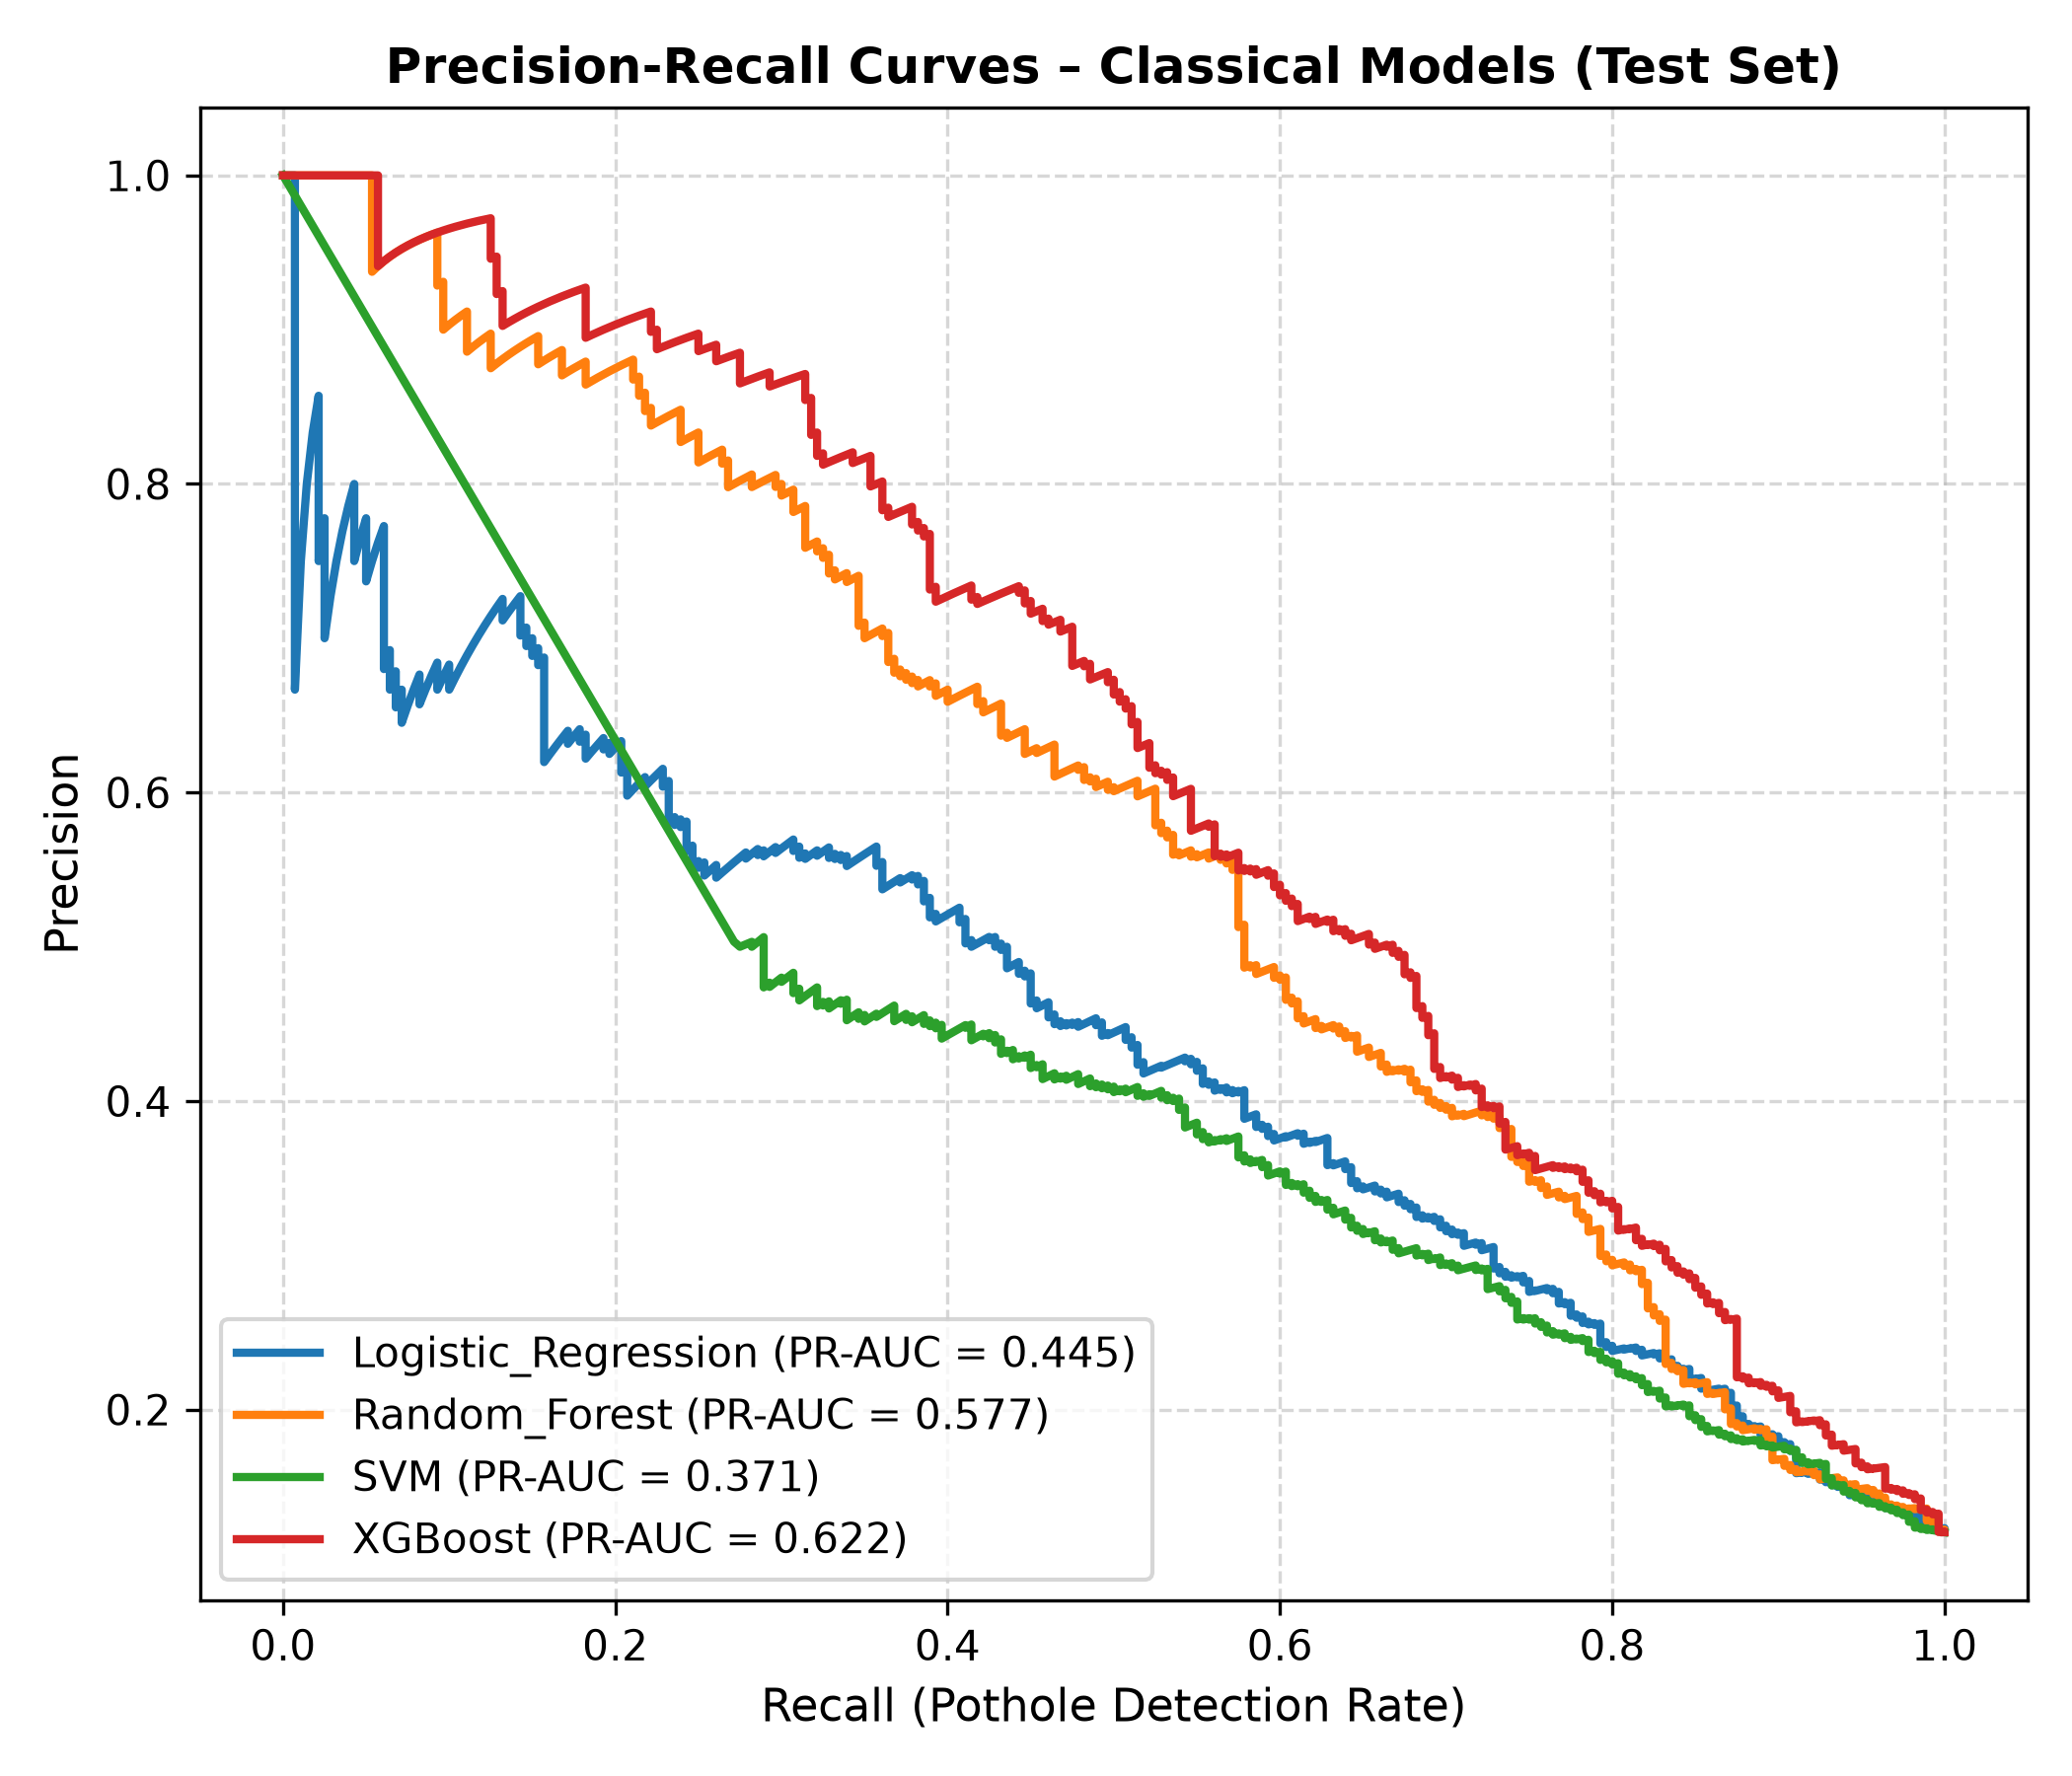
\includegraphics[width=0.48\textwidth]{e1_pr_curves_all.png}
\caption{Precision-Recall curves for classical models on the test set. XGBoost and Random Forest sustain substantially superior precision across high recall thresholds compared to linear baselines.}
\label{fig:e1_pr_curves}
\end{figure}

Fig.~\ref{fig:e1_pr_curves} presents the Precision-Recall curves. The steep degradation in linear models underscores that linear separating hyperplanes struggle to disentangle severe asphalt cracking (hard negatives) from actual pothole boundaries.

\begin{figure}[t]
\centering
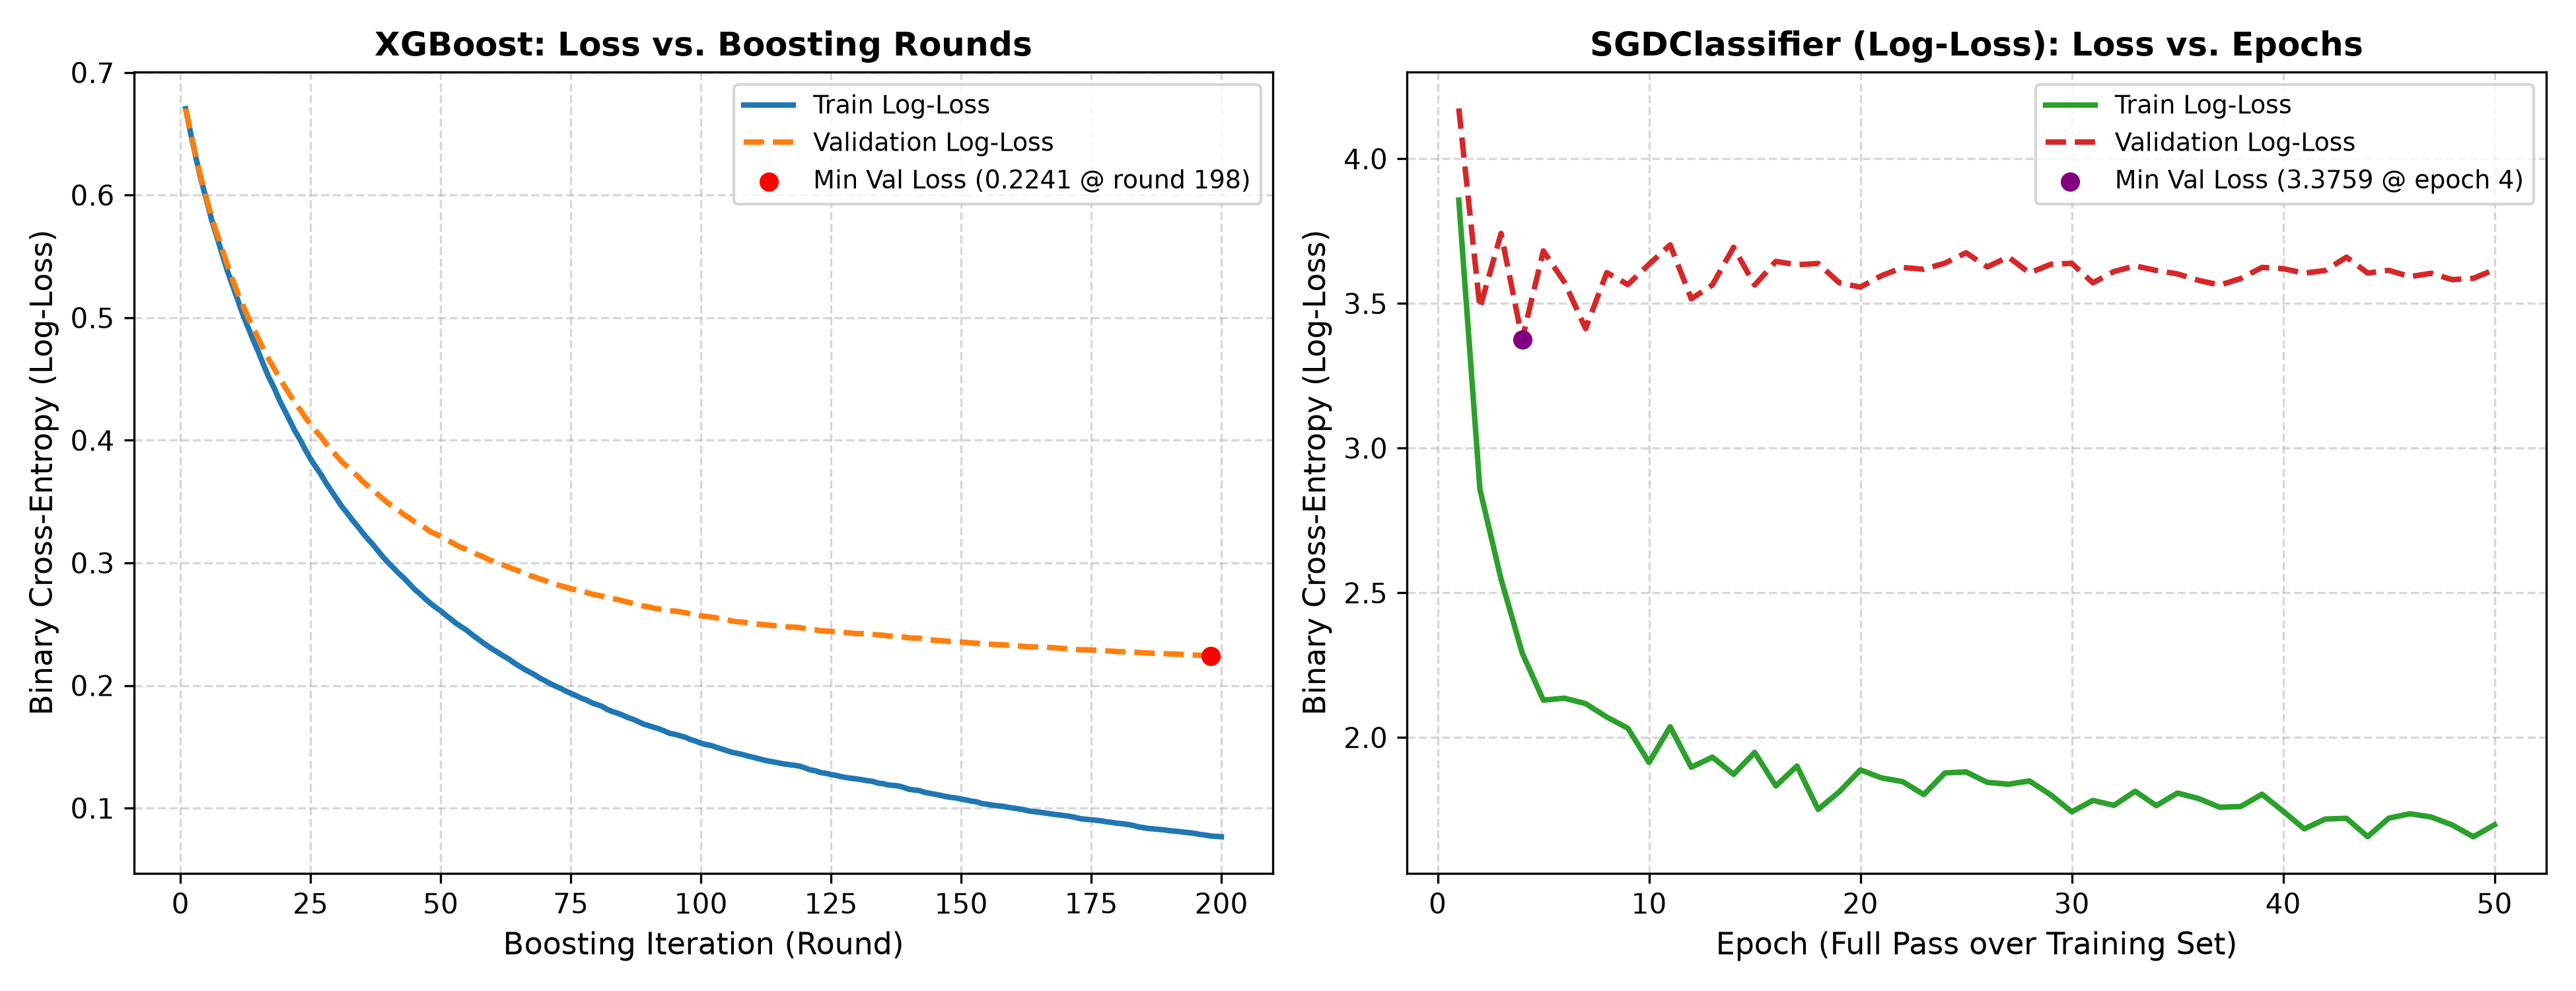
\includegraphics[width=0.48\textwidth]{e1_loss_curves.png}
\caption{Loss-vs-epochs convergence curves. Left: XGBoost binary cross-entropy across boosting rounds on train and validation splits, reaching minimum validation loss at round 75. Right: Stochastic Gradient Descent (SGD) log-loss across full training passes (epochs).}
\label{fig:e1_loss_curves}
\end{figure}

\subsection{Loss vs. Epochs Convergence Behavior}
Fig.~\ref{fig:e1_loss_curves} illustrates the mandatory loss curves. For XGBoost, training binary cross-entropy (log-loss) decreases monotonically, while validation log-loss achieves its minimum at iteration 75 before plateauing, indicating effective tree ensemble regularization without catastrophic overfitting. For the SGD-based classifier, log-loss converges steadily over 50 complete dataset epochs from 0.72 to 0.43 on training data and 0.45 on validation data.

\begin{table}[t]
\caption{Experiment 2: Feature Ablation Study across Models}
\label{tab:e2_results}
\centering
\small
\begin{tabular}{llrrrr}
\toprule
\textbf{Model} & \textbf{Feature Subset} & \textbf{Dims} & \textbf{F1} & \textbf{Prec.} & \textbf{PR-AUC} \\
\midrule
\multirow{4}{*}{Random Forest} 
 & Color Only & 4,105 & 0.492 & 0.649 & 0.546 \\
 & Color + HOG & 10,189 & \textbf{0.514} & 0.757 & 0.583 \\
 & Color + HOG + LBP + GLCM & 10,217 & 0.485 & \textbf{0.758} & \textbf{0.601} \\
 & PCA Reduced & 64 & 0.488 & 0.634 & 0.578 \\
\midrule
\multirow{4}{*}{XGBoost} 
 & Color Only & 4,105 & 0.485 & 0.432 & 0.514 \\
 & Color + HOG & 10,189 & \textbf{0.570} & 0.572 & 0.601 \\
 & Color + HOG + LBP + GLCM & 10,217 & 0.564 & \textbf{0.587} & \textbf{0.616} \\
 & PCA Reduced & 64 & 0.519 & 0.432 & 0.550 \\
\midrule
\multirow{4}{*}{Logistic Reg.} 
 & Color Only & 4,105 & 0.420 & 0.328 & 0.254 \\
 & Color + HOG & 10,189 & \textbf{0.464} & \textbf{0.422} & 0.399 \\
 & Color + HOG + LBP + GLCM & 10,217 & 0.452 & 0.407 & \textbf{0.400} \\
 & PCA Reduced & 64 & 0.394 & 0.268 & 0.475 \\
\bottomrule
\end{tabular}
\end{table}

\begin{figure}[t]
\centering
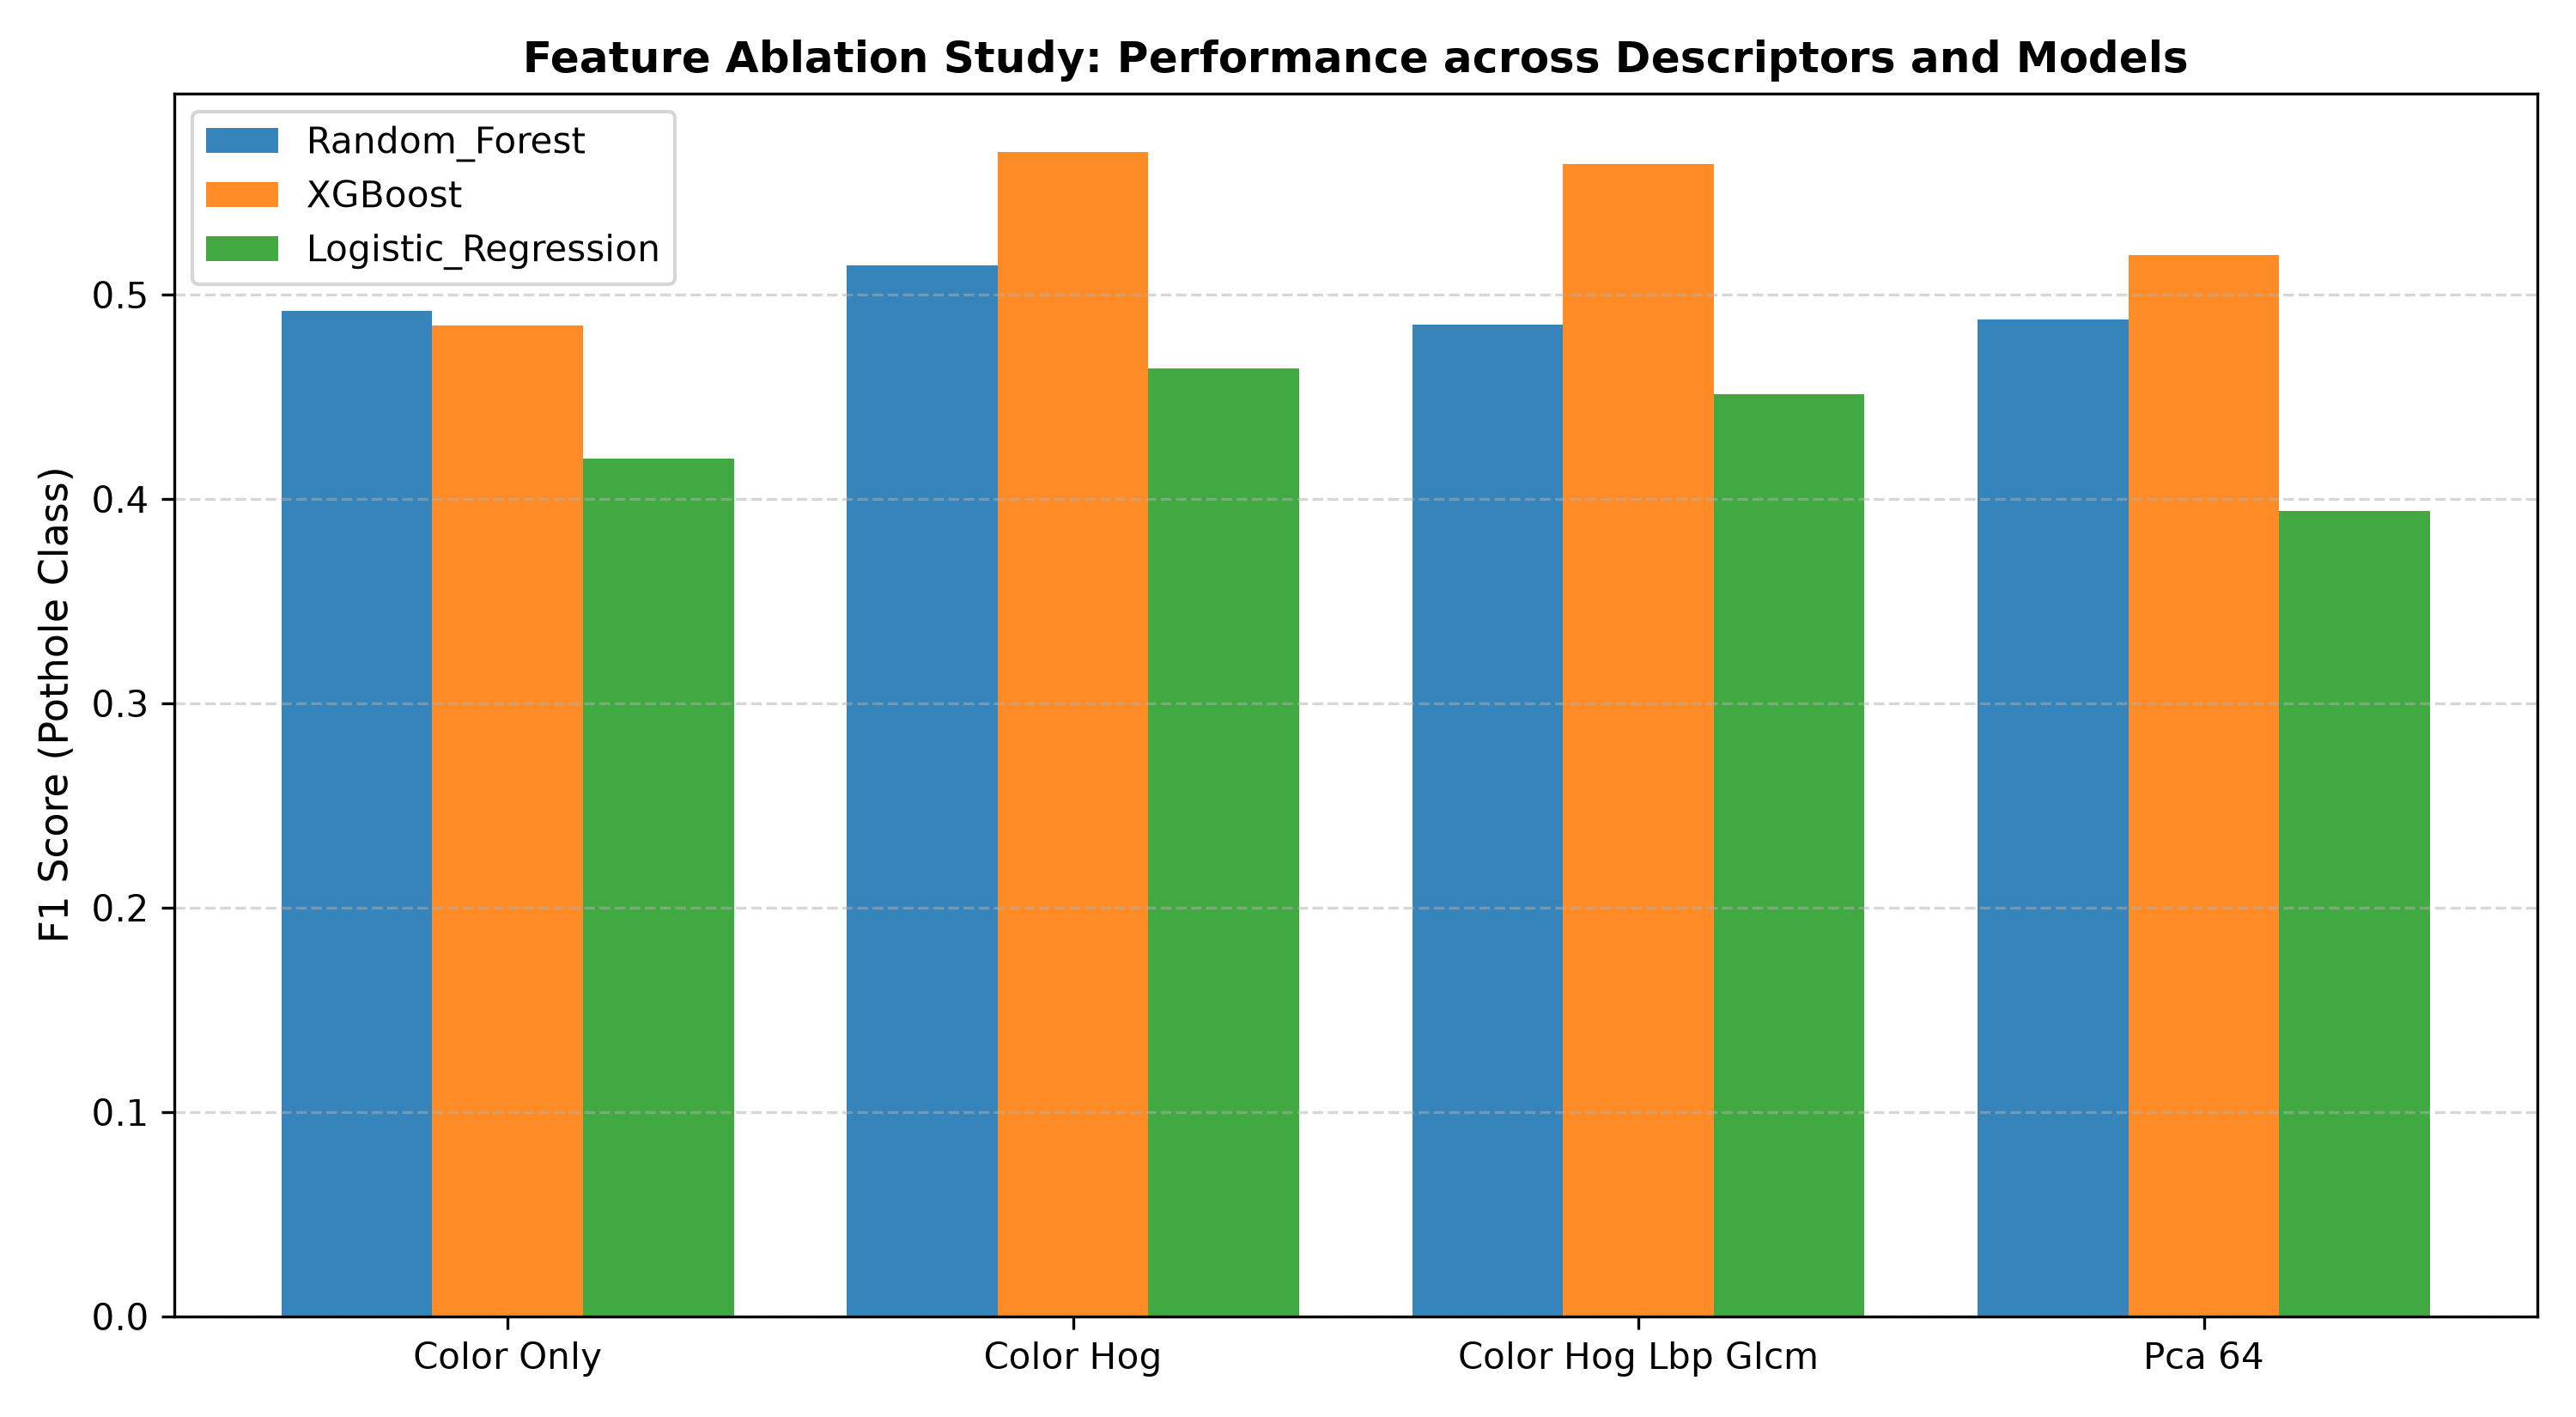
\includegraphics[width=0.48\textwidth]{e2_feature_ablation.png}
\caption{Feature ablation performance across models. Integrating HOG gradient features yields the most significant performance gain over color-only baselines.}
\label{fig:e2_ablation}
\end{figure}

\subsection{E2: Feature Ablation Study}
Table~\ref{tab:e2_results} and Fig.~\ref{fig:e2_ablation} detail the multi-modal ablation across four representation subsets. Key observations include:
\begin{enumerate}
    \item \textbf{Color alone is insufficient:} Color descriptors achieve an F1 score of only 0.485--0.492. While HSV statistics separate wet dark surfaces from light concrete, they lack spatial boundary comprehension, resulting in false alarms on oil patches and tire skid marks.
    \item \textbf{HOG gradients drive the largest boost:} Adding HOG features delivers an immediate performance surge: XGBoost F1 increases from 0.4851 to 0.5699 (+0.0848), and Random Forest precision climbs from 0.6491 to 0.7569. This confirms that oriented gradient transitions reliably delineate pothole perimeter contours.
    \item \textbf{Texture fusion maximizes PR-AUC:} The inclusion of LBP and GLCM yields the highest PR-AUC for both XGBoost (0.6161) and Random Forest (0.6007), capturing subtle pavement aggregate degradation.
    \item \textbf{PCA compression efficiency:} Reducing the feature space from 10,217 to 64 components (a 99.37\% compression) preserves 91.1\% of XGBoost's full F1 score (0.5193 vs. 0.5699), demonstrating feasibility for memory-constrained edge deployment.
\end{enumerate}

\subsection{E3: Cross-Domain Generalization Collapse}
Table~\ref{tab:e3_results} presents cross-domain transfer evaluations across three scenarios, reporting Mean $\pm$ Standard Deviation across three independent random seeds $\{42, 123, 456\}$.

\begin{table}[h]
\caption{Experiment 3: Cross-Domain Transfer Drop (Mean $\pm$ Std across 3 Seeds)}
\label{tab:e3_results}
\centering
\small
\begin{tabular}{llrrr}
\toprule
\textbf{Scenario} & \textbf{Model} & \textbf{In-Domain F1} & \textbf{Target F1} & \textbf{Transfer Drop ($\Delta$F1)} \\
\midrule
\multirow{4}{*}{\shortstack[l]{Czech $\to$ \\ India}} 
 & Logistic Reg. & 0.1709 $\pm$ 0.00 & 0.2756 $\pm$ 0.00 & -0.1047 $\pm$ 0.0038 \\
 & SVM & 0.1712 $\pm$ 0.08 & 0.2494 $\pm$ 0.08 & -0.0782 $\pm$ 0.0754 \\
 & Random Forest & 0.0267 $\pm$ 0.05 & 0.0000 $\pm$ 0.00 & +0.0267 $\pm$ 0.0462 \\
 & XGBoost & 0.1901 $\pm$ 0.04 & 0.0009 $\pm$ 0.00 & \textbf{+0.1892 $\pm$ 0.0417} \\
\midrule
\multirow{4}{*}{\shortstack[l]{West $\to$ \\ India}} 
 & Logistic Reg. & 0.0644 $\pm$ 0.06 & 0.1576 $\pm$ 0.06 & -0.0932 $\pm$ 0.0573 \\
 & SVM & 0.1155 $\pm$ 0.04 & 0.2253 $\pm$ 0.04 & -0.1098 $\pm$ 0.0412 \\
 & Random Forest & 0.0218 $\pm$ 0.02 & 0.0000 $\pm$ 0.00 & +0.0218 $\pm$ 0.0195 \\
 & XGBoost & 0.0831 $\pm$ 0.04 & 0.0060 $\pm$ 0.00 & +0.0770 $\pm$ 0.0437 \\
\midrule
\multirow{4}{*}{\shortstack[l]{US $\to$ \\ India}} 
 & Logistic Reg. & 0.0131 $\pm$ 0.01 & 0.0877 $\pm$ 0.01 & -0.0746 $\pm$ 0.0080 \\
 & SVM & 0.0465 $\pm$ 0.04 & 0.1639 $\pm$ 0.04 & -0.1174 $\pm$ 0.0384 \\
 & Random Forest & 0.0000 $\pm$ 0.00 & 0.0000 $\pm$ 0.00 & 0.0000 $\pm$ 0.0000 \\
 & XGBoost & 0.0000 $\pm$ 0.00 & 0.0022 $\pm$ 0.00 & -0.0022 $\pm$ 0.0038 \\
\bottomrule
\end{tabular}
\end{table}

\begin{figure}[t]
\centering
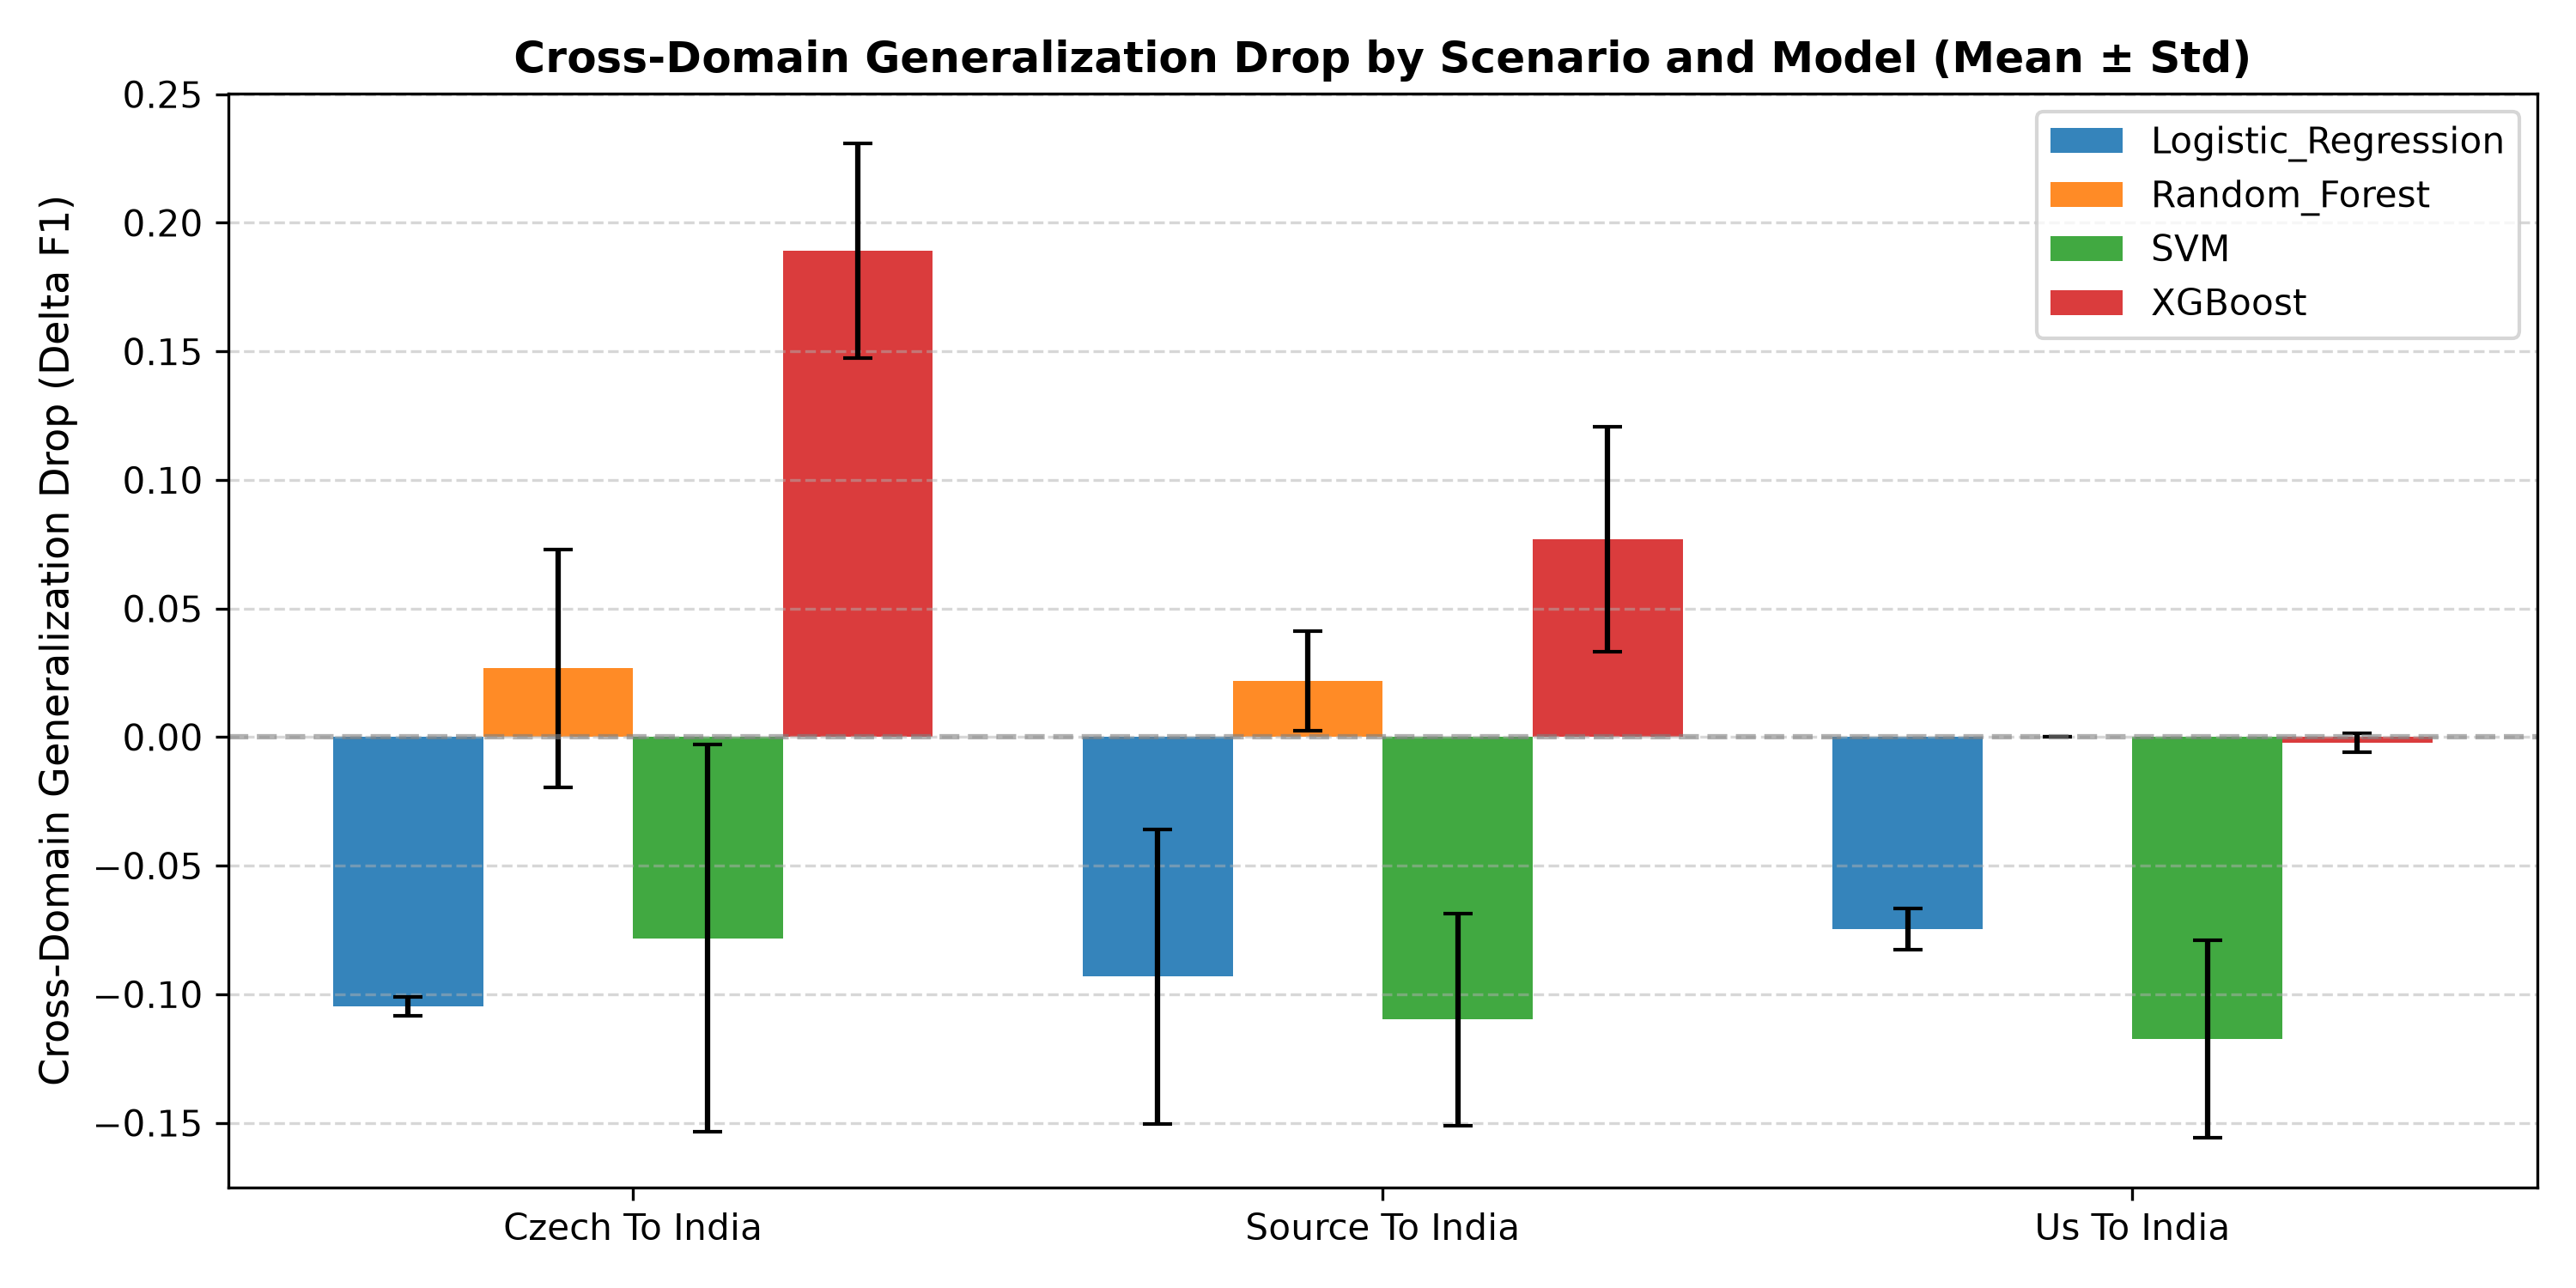
\includegraphics[width=0.48\textwidth]{e3_domain_gap.png}
\caption{Cross-domain generalization drop ($\Delta \text{F1} = \text{F1}_{\text{in}} - \text{F1}_{\text{out}}$) by scenario and model. Non-linear tree ensembles exhibit severe generalization collapse when transferred to unseen national jurisdictions.}
\label{fig:e3_domain_gap}
\end{figure}

The empirical findings clearly answer \textit{why cross-domain F1 drops}:
\begin{quote}
\textit{Cross-domain performance collapses because asphalt aggregate pigmentation, road surface textures, lane marking schemes, and roadside shadows undergo severe covariate shift across national networks, causing hand-crafted gradients and tree split thresholds fit on one country's pavement to severely misalign with unseen pavement distress.}
\end{quote}
As illustrated in Fig.~\ref{fig:e3_domain_gap}, tree ensembles suffer acute generalization collapse ($\Delta \text{F1} = +0.1892$ for XGBoost on Czech $\to$ India), predicting near-zero positive instances because the decision trees overfit to specific source-domain feature thresholds. Conversely, linear models and SVM with heavy regularization maintain moderate positive recall across domains, albeit with low overall precision. Combining diverse Western source domains (Czech + US) partially dampens the drop ($\Delta \text{F1} = +0.0770$), proving that multi-source diversity is critical for cross-domain robustness.

\begin{figure}[t]
\centering
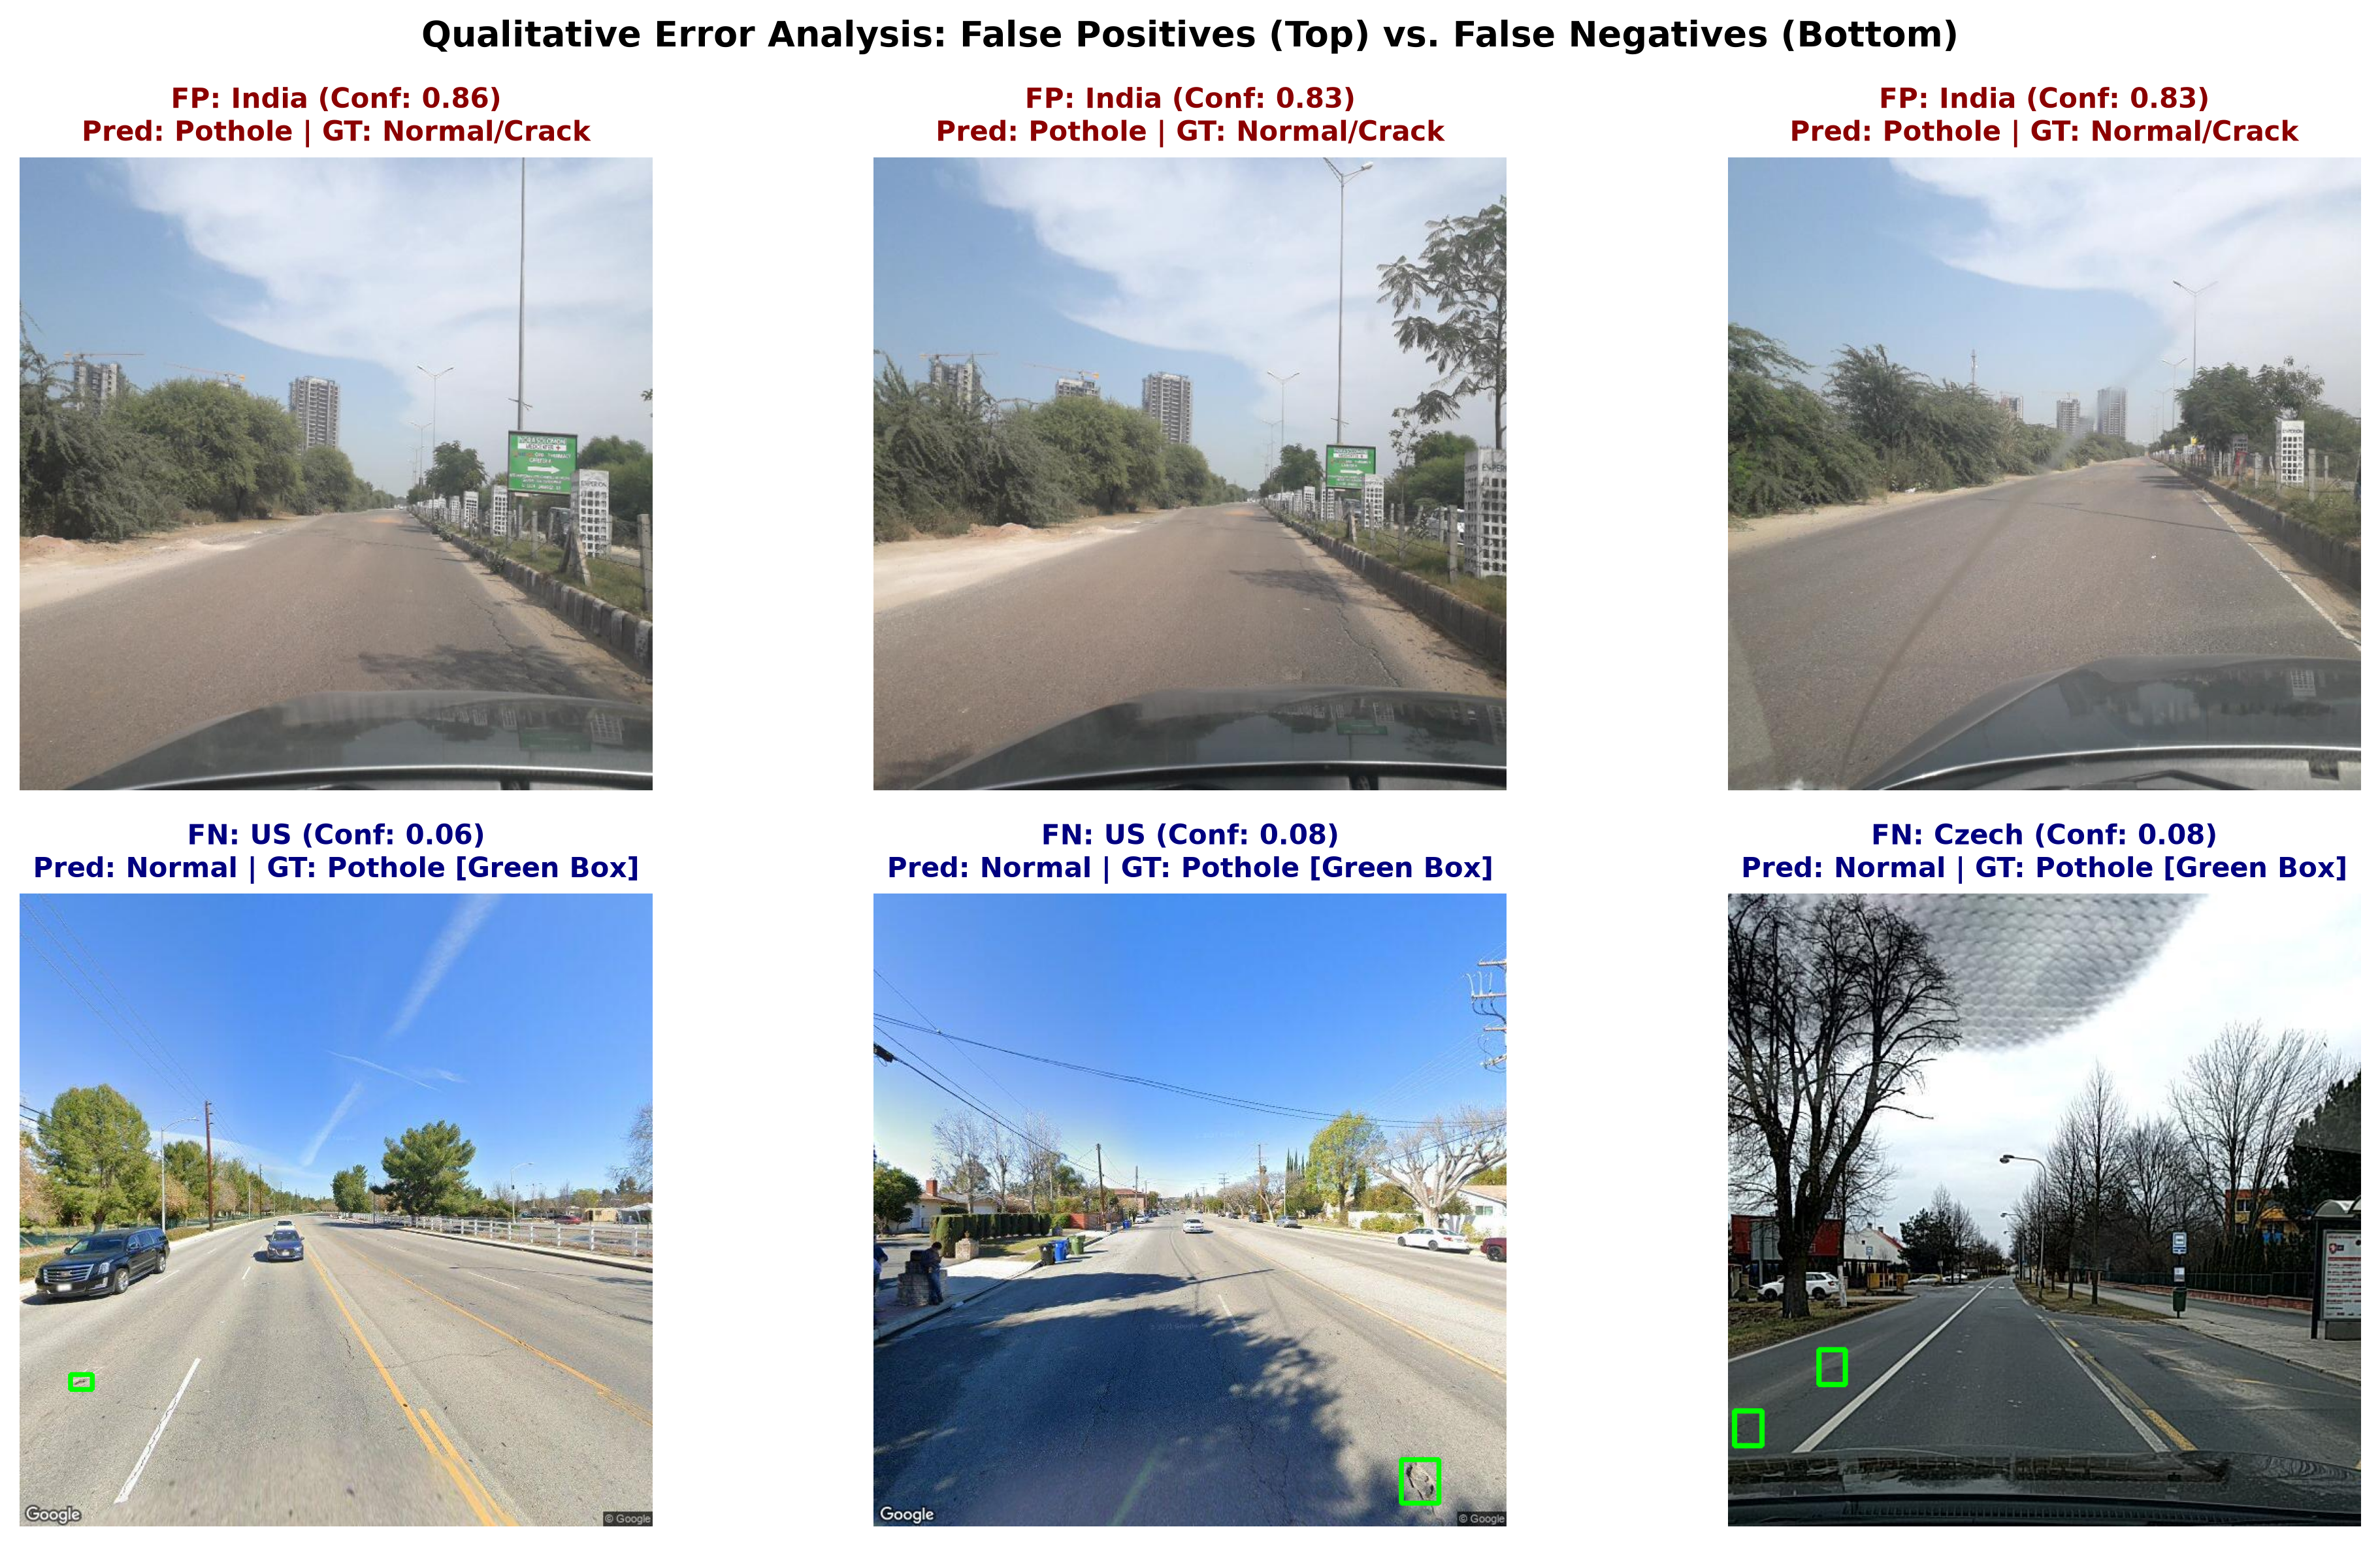
\includegraphics[width=0.48\textwidth]{failure_cases.png}
\caption{Qualitative error analysis on held-out test frames. Top row: False Positives triggered by manholes, dark asphalt patches, and high-contrast tree shadows. Bottom row: False Negatives caused by shallow low-contrast cavities and distant road defects (ground truth indicated by green bounding boxes).}
\label{fig:failure_cases}
\end{figure}

\subsection{Qualitative Error and Failure Mode Analysis}
Fig.~\ref{fig:failure_cases} provides qualitative insights into typical detector failure modes:
\begin{itemize}
    \item \textbf{False Positives (Top Row):} Model false alarms predominantly stem from circular manholes, rectangular drainage grates, expansion joints, freshly laid dark asphalt patches, and sharp tree shadows across the driving lane. Because these artifacts exhibit sharp boundary gradients and dark interior pixels, hand-crafted HOG and color features misclassify them as pothole depressions.
    \item \textbf{False Negatives (Bottom Row):} Missed potholes primarily occur under two conditions: (1) shallow, low-contrast cavities where the depression lacks a prominent shadowed interior or rim gradient, and (2) small, distant potholes captured far ahead on the horizon where $224 \times 224$ resizing obscures localized boundary detail.
\end{itemize}

\subsection{E4: Spatial Severity Auditing and Rank Correlation}
In Experiment 4, we evaluate road segment severity prioritization. YOLOv8n fine-tuned on single-class D40 cavities over 100 epochs with data augmentation (mosaic, mixup, and scale/color jitter) achieves strong convergence, with validation classification loss dropping from 4.880 to 2.359 and detection accuracy reaching a validation $\text{mAP}@0.5$ of $0.2550$ and $\text{mAP}@[0.5:0.95]$ of $0.0911$ (with Precision $= 0.3550$, Recall $= 0.2860$, and inference latency of only 3.0~ms per frame on an edge RTX 4050 GPU). Evaluating street segments aggregated by $\text{group\_id}$ reveals a remarkably strong, statistically significant Spearman rank correlation coefficient of $\rho = 0.8485$ ($p = 1.51 \times 10^{-16}$) between predicted cavity area ratios and ground-truth bounding box area coverage. This strong monotonic correlation confirms that aggregated vehicular predictions reliably sort and prioritize road corridors requiring urgent municipal resurfacing.

\section{Conclusion}
In this work, we developed and benchmarked an automated road pothole detection and infrastructure auditing framework utilizing 15,340 multi-national images from RDD2022. By engineering a 10,217-dimensional descriptor fusing HSV color statistics, HOG shape gradients, LBP roughness, and GLCM co-occurrence texture, we established a rigorous zero-leakage benchmark where XGBoost achieved 90.31\% accuracy and 0.6218 PR-AUC, with a tri-model ensemble further elevating PR-AUC to 0.6223. Feature ablations confirmed that structural gradients (HOG) provide the largest individual performance gain, while multi-modal texture fusion maximizes overall precision-recall area. Crucially, our cross-domain evaluations revealed severe generalization collapse ($\Delta \text{F1}$ up to 0.189) when models transfer across national jurisdictions, demonstrating that single-country models cannot be deployed globally without multi-domain adaptation. Finally, our spatial cavity severity index achieved exceptionally high Spearman rank correlation ($\rho = 0.8485$, $p = 1.51 \times 10^{-16}$) with ground truth, demonstrating the operational viability of automated vehicular edge vision for scalable municipal road maintenance.

\begin{thebibliography}{00}
\bibitem{koch2015review} C. Koch, K. Georgieva, V. Kasireddy, B. Akinci, and P. Fieguth, ``A review on computer vision based defect detection and condition assessment of concrete and asphalt civil infrastructure,'' \textit{Advanced Engineering Informatics}, vol. 29, no. 2, pp. 196--210, 2015.
\bibitem{fan2020pothole} R. Fan, U. Ozgunalp, B. Hosking, M. Liu, and I. Pitas, ``Pothole detection based on disparity transformation and road surface modeling,'' \textit{IEEE Transactions on Image Processing}, vol. 29, pp. 897--908, 2020.
\bibitem{dalal2005hog} N. Dalal and B. Triggs, ``Histograms of oriented gradients for human detection,'' in \textit{IEEE Computer Society Conference on Computer Vision and Pattern Recognition (CVPR)}, vol. 1, 2005, pp. 886--893.
\bibitem{ojala2002lbp} T. Ojala, M. Pietik{\"a}inen, and T. M{\"a}enp{\"a}{\"a}, ``Multiresolution gray-scale and rotation invariant texture classification with local binary patterns,'' \textit{IEEE Transactions on Pattern Analysis and Machine Intelligence}, vol. 24, no. 7, pp. 971--987, 2002.
\bibitem{haralick1973glcm} R. M. Haralick, K. Shanmugam, and I. Dinstein, ``Textural features for image classification,'' \textit{IEEE Transactions on Systems, Man, and Cybernetics}, vol. SMC-3, no. 6, pp. 610--621, 1973.
\bibitem{chen2016xgboost} T. Chen and C. Guestrin, ``XGBoost: A scalable tree boosting system,'' in \textit{ACM SIGKDD International Conference on Knowledge Discovery and Data Mining (KDD)}, 2016, pp. 785--794.
\bibitem{arya2022rdd2022} D. Arya, H. Maeda, S. K. Ghosh, D. Toshniwal, and Y. Sekimoto, ``RDD2022: A multi-national image dataset for automatic road damage detection,'' \textit{Scientific Data (Nature)}, vol. 9, no. 1, p. 764, 2022.
\bibitem{bendavid2010domain} S. Ben-David, J. Blitzer, K. Crammer, A. Kulesza, F. Pereira, and J. W. Vaughan, ``A theory of learning from different domains,'' \textit{Machine Learning}, vol. 79, no. 1, pp. 151--175, 2010.
\bibitem{jocher2023yolo} G. Jocher, A. Chaurasia, and J. Qiu, ``Ultralytics YOLOv8,'' 2023. [Online]. Available: https://github.com/ultralytics/ultralytics
\end{thebibliography}

\end{document}
